\section{Introduction to the Laplace Transform}

\noindent
\boxit{Definition of the Laplace Transform}

\noindent
To define the Laplace transform, we first recall the definition of an
improper integral. If $g$ is integrable over the
interval $[a,T]$ for every $T>a$, then the {\color{blue}\it improper
integral of
$g$ over\/} $[a,\infty)$ is defined as
\begin{equation} \label{eq:8.1.1}
\int^\infty_a g(t)\,dt=\lim_{T\to\infty}\int^T_a g(t)\,dt.
\end{equation}
We say that the improper integral {\color{blue}\it converges\/} if the limit in
\eqref{eq:8.1.1} exists;   otherwise, we say that the improper integral
{\color{blue}\it
diverges\/} or {\color{blue}\it does not exist\/}. Here's the definition of
the Laplace transform of a function $f$.

\begin{definition}\color{blue}\label{thmtype:8.1.1}\rm
Let $f$ be defined for $t\ge0$ and let $s$ be a real number. Then the
\href{https://mathshistory.st-andrews.ac.uk/Biographies/Laplace/}
{\color{blue}\it Laplace transform} of $f$ is the function $F$ defined by
\begin{equation}\label{eq:8.1.2} F(s)=\int_0^\infty e^{-st} f(t)\,dt,
\end{equation} for those values of $s$ for which the improper integral
converges.
\end{definition}

It is important to keep in mind that the variable of integration in
\eqref{eq:8.1.2} is $t$, while $s$ is a parameter independent of $t$. We
use $t$ as the independent variable for $f$ because in applications
the Laplace transform is usually applied to functions of time.

The Laplace transform can be viewed as an operator ${\cal L}$ that
transforms the function $f=f(t)$  into the function $F=F(s)$. Thus,
\eqref{eq:8.1.2} can be expressed as
$$
F={\cal L}(f).
$$
The functions $f$ and $F$ form a {\color{blue}\it transform pair\/}, which we'll
sometimes denote by
$$
f(t)\leftrightarrow F(s).
$$
It can be shown that if $F(s)$ is defined for $s=s_0$ then it's defined
for all $s>s_0$ (Exercise~\ref{exer:8.1.14}\part{b}).

\boxit{Computation of Some Simple Laplace Transforms}

\begin{example}\label{example:8.1.1}\rm
 Find the Laplace transform of  $f(t)=1$.
\end{example}

\solution
 From  \eqref{eq:8.1.2} with $f(t)=1$,
$$
F(s)=\int_0^\infty e^{-st}\,dt=\lim_{T\to\infty}\int_0^T e^{-st}\,
dt.
$$
If $s\ne 0$ then
\begin{equation}\label{eq:8.1.3}
\int_0^T e^{-st}dt=-{1\over s}e^{-st}\Big|_0^T={1-e^{-sT}\over s}.
\end{equation}
Therefore
\begin{equation}\label{eq:8.1.4}
\lim_{T\to\infty}\int_0^T e^{-st}dt=\left\{\begin{array}{rr}
\dst{1\over s}, &   s>0,\\
\infty, &  s<0.
\end{array}\right.
\end{equation}
If $s=0$  the integrand reduces to the constant $1$, and
$$
\lim_{T\to\infty}\int_0^T 1\,dt=\lim_{T\to\infty}\int_0^T 1\,dt=
\lim_{T\to\infty}T=\infty.
$$
Therefore $F(0)$ is undefined, and
$$
F(s)=\int_0^\infty e^{-st}dt={1\over s},\quad s>0.
$$
This result can be written in operator notation as
$$
{\cal L}(1)={1\over s},\quad s>0,
$$
or as the transform pair
$$
1\leftrightarrow{1\over s},\quad s>0.
$$

\color{blue}
\remark{
It is convenient to combine the steps of integrating from $0$ to $T$
and letting $T\to\infty$. Therefore, instead of writing \eqref{eq:8.1.3}
and \eqref{eq:8.1.4} as separate steps we write
$$
\int_0^\infty e^{-st}dt=- {1\over s} e^{-st}\Big|_0^\infty=
\left\{\begin{array}{rr}\dst{1\over s}, & s>0,\\\infty,&s<
0.\end{array}\right.
$$
We'll follow this practice throughout this chapter.}
\color{black}

\begin{example}\label{example:8.1.2}\rm
 Find the Laplace transform of $f(t)=t$.
\end{example}

\solution
  From  \eqref{eq:8.1.2} with $f(t)=t$,
\begin{equation}\label{eq:8.1.5}
F(s)=\int_0^\infty e^{-st}t\,dt.
\end{equation}
If $s\ne0$,  integrating by parts yields
\begin{eqnarray*}
\int_0^\infty e^{-st}t\,dt&=&-{te^{-st}\over s}\bigg|_0^\infty
+{1\over s}\int_0^\infty e^{-st}\,dt
=-\left[{t\over s}+{1\over s^2}\right]e^{-st}\bigg|_0^\infty
\\&=&\left\{\begin{array}{rr}\dst{1\over s^2},\quad s>0,\\
\infty,\,s<0.\end{array}\right.
\end{eqnarray*}
If $s=0$, the integral in  \eqref{eq:8.1.5} becomes
$$
\int_0^\infty t\,dt={t^2\over2}\bigg|_0^\infty=\infty.
$$
Therefore $F(0)$ is undefined and
$$
F(s)={1\over s^2},\quad s>0.
$$
This result can also be written as
$$
{\cal L}(t)={1\over s^2},\quad s>0,
$$
or as the transform pair
$$
t\leftrightarrow{1\over s^2},\quad s>0.
$$

\begin{example}\label{example:8.1.3}\rm
 Find the Laplace transform of $f(t)=e^{at}$, where $a$ is a constant.
\end{example}

\solution
From  \eqref{eq:8.1.2} with $f(t)=e^{at}$,
$$
F(s)=\int_0^\infty e^{-st}e^{at}\,dt.
$$
Combining the exponentials yields
$$
F(s)=\int_0^\infty e^{-(s-a)t}\,dt.
$$
However, we know from Example~\ref{example:8.1.1}  that
$$
\int_0^\infty e^{-st}\,dt={1\over s},\quad s>0.
$$
Replacing $s$ by $s-a$ here shows that
$$
F(s)={1\over s-a},\quad s>a.
$$
This can also be written as
$$
{\cal L}(e^{at})={1\over s-a},\quad s>a, \text{\; or \; }
 e^{at}\leftrightarrow{1\over s-a},\quad s>a.
$$

\begin{example}\label{example:8.1.4}\rm
Find the Laplace transforms of $f(t)=\sin\omega t$ and
$g(t)=\cos\omega t$, where $\omega$ is a constant.
\end{example}

\solution  Define
\begin{equation}\label{eq:8.1.6}
F(s)=\int_0^\infty e^{-st}\sin\omega t\,dt
\end{equation}
and
\begin{equation}\label{eq:8.1.7}
G(s)=\int_0^\infty e^{-st}\cos\omega t\,dt.
\end{equation}
If $s>0$, integrating  \eqref{eq:8.1.6} by parts yields
$$
F(s)=-{e^{-st}\over s}\sin\omega t\Big|_0^\infty+{\omega\over s}
\int_0^\infty e^{-st}\cos\omega t\,dt,
$$
so
\begin{equation}\label{eq:8.1.8}
F(s)={\omega\over s}G(s).
\end{equation}
If $s>0$, integrating  \eqref{eq:8.1.7} by parts yields
$$
G(s)=-{e^{-st}\cos\omega t\over s}\Big|_0^\infty - {\omega\over s}
\int_0^\infty e^{-st}\sin\omega t\,dt,
$$
so
$$
G(s)={1\over s} - {\omega\over s} F(s).
$$
Now substitute from  \eqref{eq:8.1.8} into this to obtain
$$
G(s)={1\over s} - {\omega^2\over s^2} G(s).
$$
Solving this for $G(s)$ yields
$$
G(s)={s\over s^2+\omega^2},\quad s>0.
$$
This and  \eqref{eq:8.1.8} imply that
$$
F(s)={\omega\over s^2+\omega^2},\quad s>0.
$$

\boxit{Tables of Laplace transforms}

\noindent
Extensive tables of Laplace transforms have been compiled and are
commonly used in applications. The brief table of Laplace transforms
in the Appendix will be adequate for our
purposes.

\begin{example}\label{example:8.1.5}\rm  Use the
table of Laplace transforms to find  ${\cal L}(t^3e^{4t})$.
\end{example}

\solution  The table
includes the transform pair
$$
t^ne^{at}\leftrightarrow {n!\over(s-a)^{n+1}}.
$$
Setting $n=3$  and $a=4$ here yields
$$
{\cal L}(t^3e^{4t})={3!\over(s-4)^4}={6\over(s-4)^4}.\bbox
$$

We'll  sometimes write Laplace transforms of specific functions
without explicitly stating how they are obtained. In such cases you
should refer to the table of Laplace transforms.

\boxit{Linearity of the Laplace Transform}

\noindent
The next theorem presents an important property of the Laplace
transform.

\begin{theorem}\color{blue}$[$Linearity Property$]$\label{thmtype:8.1.2}
 Suppose ${\cal L}(f_i)$ is defined for
 $s>s_i$, $1\le i\le n)$.
Let $s_0$ be the largest of the numbers $s_1$, $s_{2}$, \dots,$s_n$, and
let
$c_1$, $c_2$,\dots, $c_n$ be  constants. Then
$$
{\cal L}(c_1f_1+c_2f_2+\cdots+c_nf_n)=c_1{\cal L}(f_1)+c_2{\cal L}(f_2)
+\cdots+c_n{\cal L}(f_n)\mbox{ for } s>s_0.
$$
\end{theorem}

\proof  We give the proof for the case where $n=2$. If $s>s_0$ then
\begin{eqnarray*}
{\cal L}(c_1f_1+c_2f_2)&=&
\int_0^\infty
e^{-st}\left(c_1f_1(t)+c_2f_2(t))\right)\,dt\\
&=&c_1\int_0^\infty e^{-st}f_1(t)\,dt+c_2\int_0^\infty e^{-st}f_2(t)\,dt\\
&=&c_1{\cal L}(f_1)+c_2{\cal L}(f_2).
\end{eqnarray*}

\begin{example}\label{example:8.1.6}\rm
Use  Theorem~\ref{thmtype:8.1.2} and the known Laplace transform
$$
{\cal L}(e^{at})={1\over s-a}
$$
 to find ${\cal L}(\cosh bt)\,(b\ne0)$.
\end{example}

\solution  By definition,
$$
\cosh bt={e^{bt}+e^{-bt}\over 2}.
$$
Therefore
\begin{equation}\label{eq:8.1.9}
\begin{array}{ccl}
{\cal L}(\cosh bt)&=& {\cal L}\left(\dst{1\over 2} e^{bt}+\dst{1\over
2}e^{-bt}\right)\\[2\jot]
&=&\dst{1\over 2} {\cal L}(e^{bt}) +\dst{1\over 2} {\cal L}(e^{-bt})
\qquad
\hbox{(linearity property)}\\[2\jot]
&=&\dst{1\over 2}\,\dst{1\over s-b} +\dst{1\over 2}\,\dst{1\over
s+b},
\end{array}
\end{equation}
where the first transform on the right is defined for $s>b$ and the
second
for $s>-b$; hence, both are defined for $s>|b|$.  Simplifying the
last expression in \eqref{eq:8.1.9} yields
$$
{\cal L}(\cosh bt)={s\over s^2-b^2},\quad s>|b|.
$$

\boxit{The First Shifting Theorem}

\noindent
The next theorem enables us to start with known transform pairs and derive
others. (For other results of this kind, see Exercises~\ref{exer:8.1.6}  and
\ref{exer:8.1.13}.)

\begin{theorem}\color{blue}$[$First Shifting
Theorem$]$\label{thmtype:8.1.3}
 If
\begin{equation}\label{eq:8.1.10}
F(s)=\int_0^\infty e^{-st} f(t)\,dt
\end{equation}
is the Laplace transform of $f(t)$ for $s>s_0$, then $F(s-a)$ is the
Laplace transform of $e^{at}f(t)$ for $s >s_0+a$.
\end{theorem}

{\sc Proof.} Replacing $s$ by $s-a$ in  \eqref{eq:8.1.10} yields
\begin{equation}\label{eq:8.1.11}
F(s-a)=\int_0^\infty e^{-(s-a)t}f(t)\,dt
\end{equation}
if $s-a>s_0$; that is, if $s>s_0+a$.  However,  \eqref{eq:8.1.11} can
be rewritten as
$$
F(s-a)=\int_0^\infty e^{-st}\left(e^{at}f(t)\right)\,dt,
$$
which implies the conclusion.

\begin{example}\label{example:8.1.7}\rm
  Use Theorem~\ref{thmtype:8.1.3} and the known Laplace
transforms of $1$, $t$, $\cos\omega t$, and $\sin\omega t$ to find
$$
{\cal L}(e^{at}),\quad {\cal L}(te^{at}),\quad {\cal L}(e^{\lambda t}\sin
\omega t),\mbox{and } {\cal L}(e^{\lambda t}\cos\omega t).
$$
\end{example}

\solution  In the following table the known
transform pairs  are listed on the left and  the required  transform pairs
listed on the right are obtained  by applying
Theorem~\ref{thmtype:8.1.3}.

\begin{center}
\begin{tabular}{|c|c|}\hline
$f(t)\leftrightarrow F(s)$ & $e^{at}f(t)\leftrightarrow F(s-a)$ \\\hline
&\\[9pt] $1\leftrightarrow\dst{1\over s},\quad s>0$ &
 $e^{at}\leftrightarrow\dst{1\over(s-a)},\quad s>a$\\[9pt]
  $t\leftrightarrow\dst{{1\over s^2}},\quad s>0$ &
$te^{at}\leftrightarrow\dst{{1\over(s-a)^2}},\quad s>a$\\[9pt]
$\sin\omega t\leftrightarrow\dst{{\omega\over
s^2+\omega^2}},\quad s>0$&
$e^{\lambda t}\sin\omega t\leftrightarrow\dst{{\omega\over
(s-\lambda)^2+\omega^2}},\,s>\lambda$\\[9pt]
$\cos\omega t\leftrightarrow\dst{{s\over
s^2+\omega^2}},\quad s>0$ &
$e^{\lambda t}\sin\omega t\leftrightarrow\dst{{s-\lambda\over
(s-\lambda)^2+\omega^2}},\,s>\lambda$\\[9pt]\hline
\end{tabular}
\end{center}

\boxit{Existence of Laplace Transforms}

\noindent
Not every function has a Laplace transform.  For example, it can be shown
(Exercise~\ref{exer:8.1.3}) that
$$
\int_0^\infty e^{-st}e^{t^2} dt=\infty
$$
for every real number $s$. Hence, the function $f(t)=e^{t^2}$ does not
have a Laplace transform.

Our next objective is to establish conditions that ensure the
existence of the Laplace transform of a function. We first review some
relevant definitions from calculus.

Recall that a limit
$$
\lim_{t\to t_0} f(t)
$$
exists if and only if the one-sided limits
$$
\lim_{t\to t_0-}f(t)\hbox{\quad and\quad}\lim_{t\to t_0+}f(t)
$$
  both exist and are equal;   in this case,
$$
\lim_{t\to t_0}f(t)=\lim_{t\to t_0-}f(t)=\lim_{t\to t_0+}f(t) .
$$
Recall also that $f$ is continuous at a point $t_0$ in an open interval
$(a,b)$ if and only if
$$
\lim_{t\to t_0}f(t)=f(t_0),
$$
which is  equivalent to
\begin{equation}\label{eq:8.1.12}
\lim_{t\to t_0+}f(t)=\lim_{t\to t_0-}f(t)=f(t_0).
\end{equation}
For simplicity, we  define
$$
f(t_0+)=\lim_{t\to t_0+}f(t)\quad\hbox{and }\quad f(t_0-)=\lim_{t\to
t_0-}f(t),
$$
so  \eqref{eq:8.1.12} can be expressed as
$$
f(t_0+)=f(t_0-)=f(t_0).
$$
If $f(t_0+)$ and $f(t_0-)$ have finite but distinct values,  we say
that $f$ has a {\color{blue}\it jump discontinuity\/}  at $t_0$,
 and
$$
f(t_0+)-f(t_0-)
$$
is called the {\color{blue}\it jump} in $f$ at $t_0$ (Figure~\ref{figure:8.1.1}).

\
\begin{figure}[tbp]
  \centering\color{blue}
  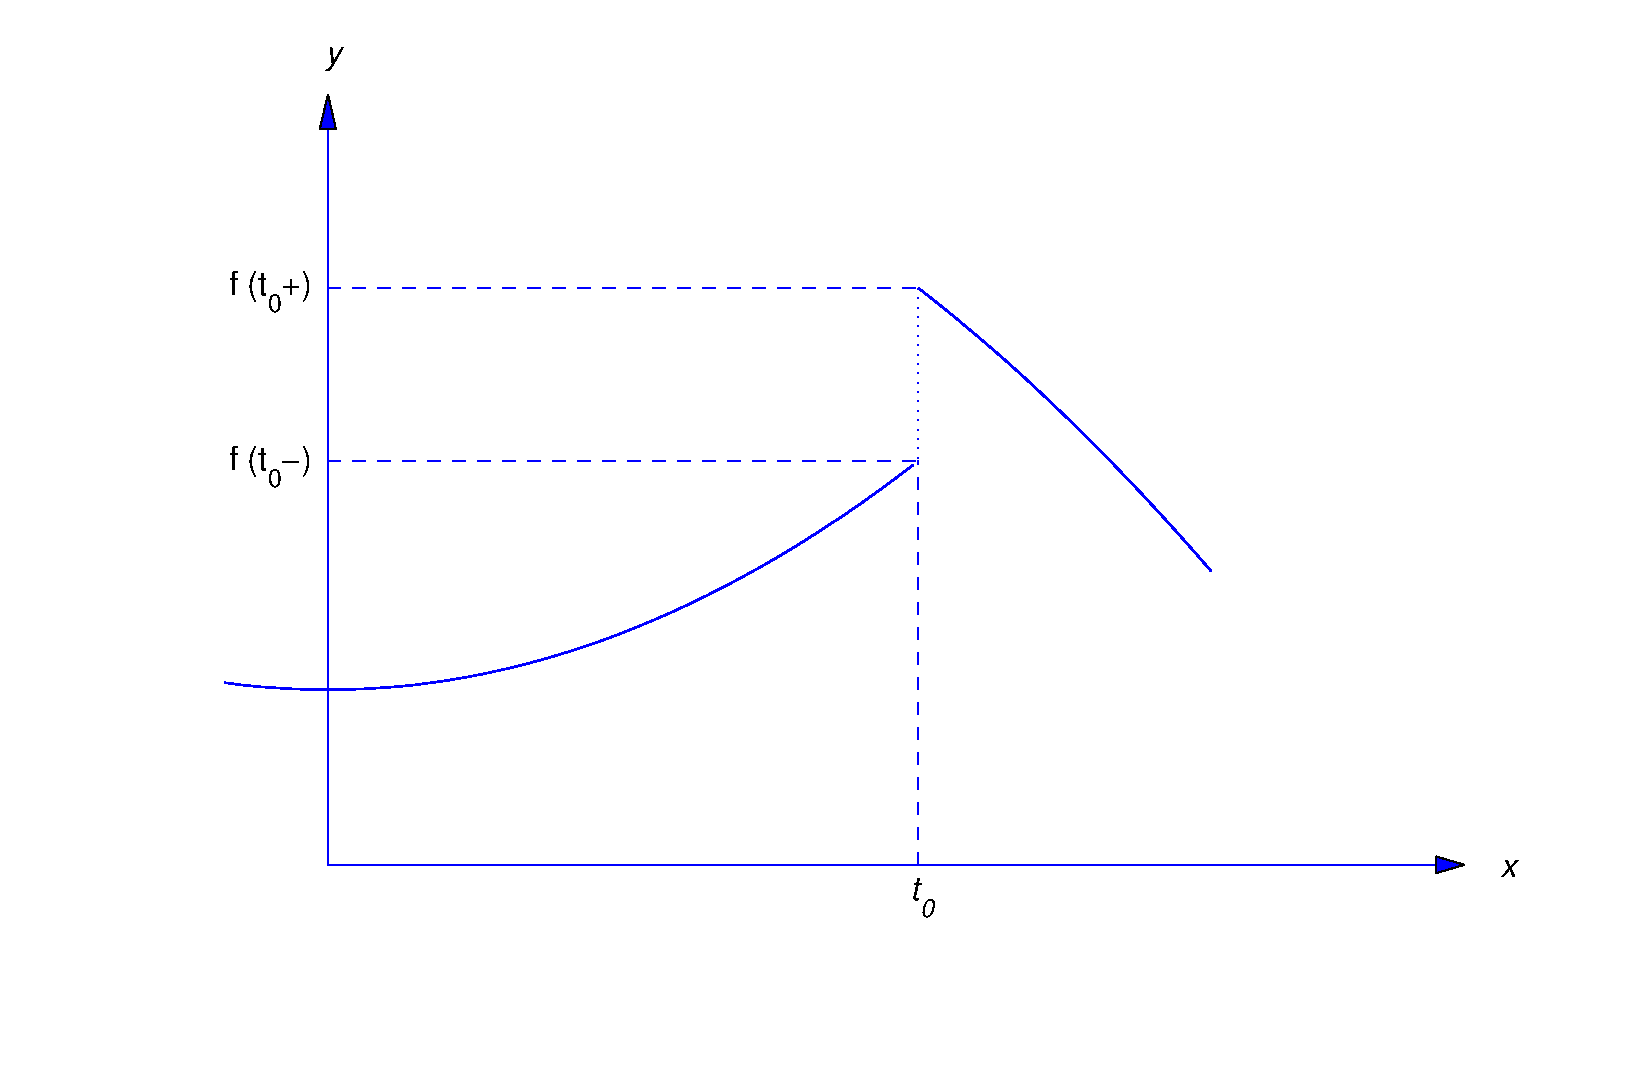
\includegraphics[bb=-78 148 689 643,width=5.67in,height=3.66in,keepaspectratio]{fig080101}
\caption{ A jump discontinuity}
  \label{figure:8.1.1}
\end{figure}

If $f(t_0+)$ and $f(t_0-)$ are finite and equal, but either $f$ isn't
defined at $t_0$ or it's defined but
$$
f(t_0)\ne f(t_0+)=f(t_0-),
$$
 we say that $f$ has a {\color{blue}\it removable discontinuity\/} at $t_0$
(Figure~\ref{figure:8.1.2}).
This terminology is appropriate since a function $f$  with a removable
discontinuity at $t_0$  can be made continuous at $t_0$ by defining (or
redefining)
$$
f(t_0)=f(t_0+)=f(t_0-).
$$

\begin{figure}[htbp]
\color{blue}
  \begin{minipage}[b]{0.5\linewidth}
    \centering
   \scalebox{.65}{
  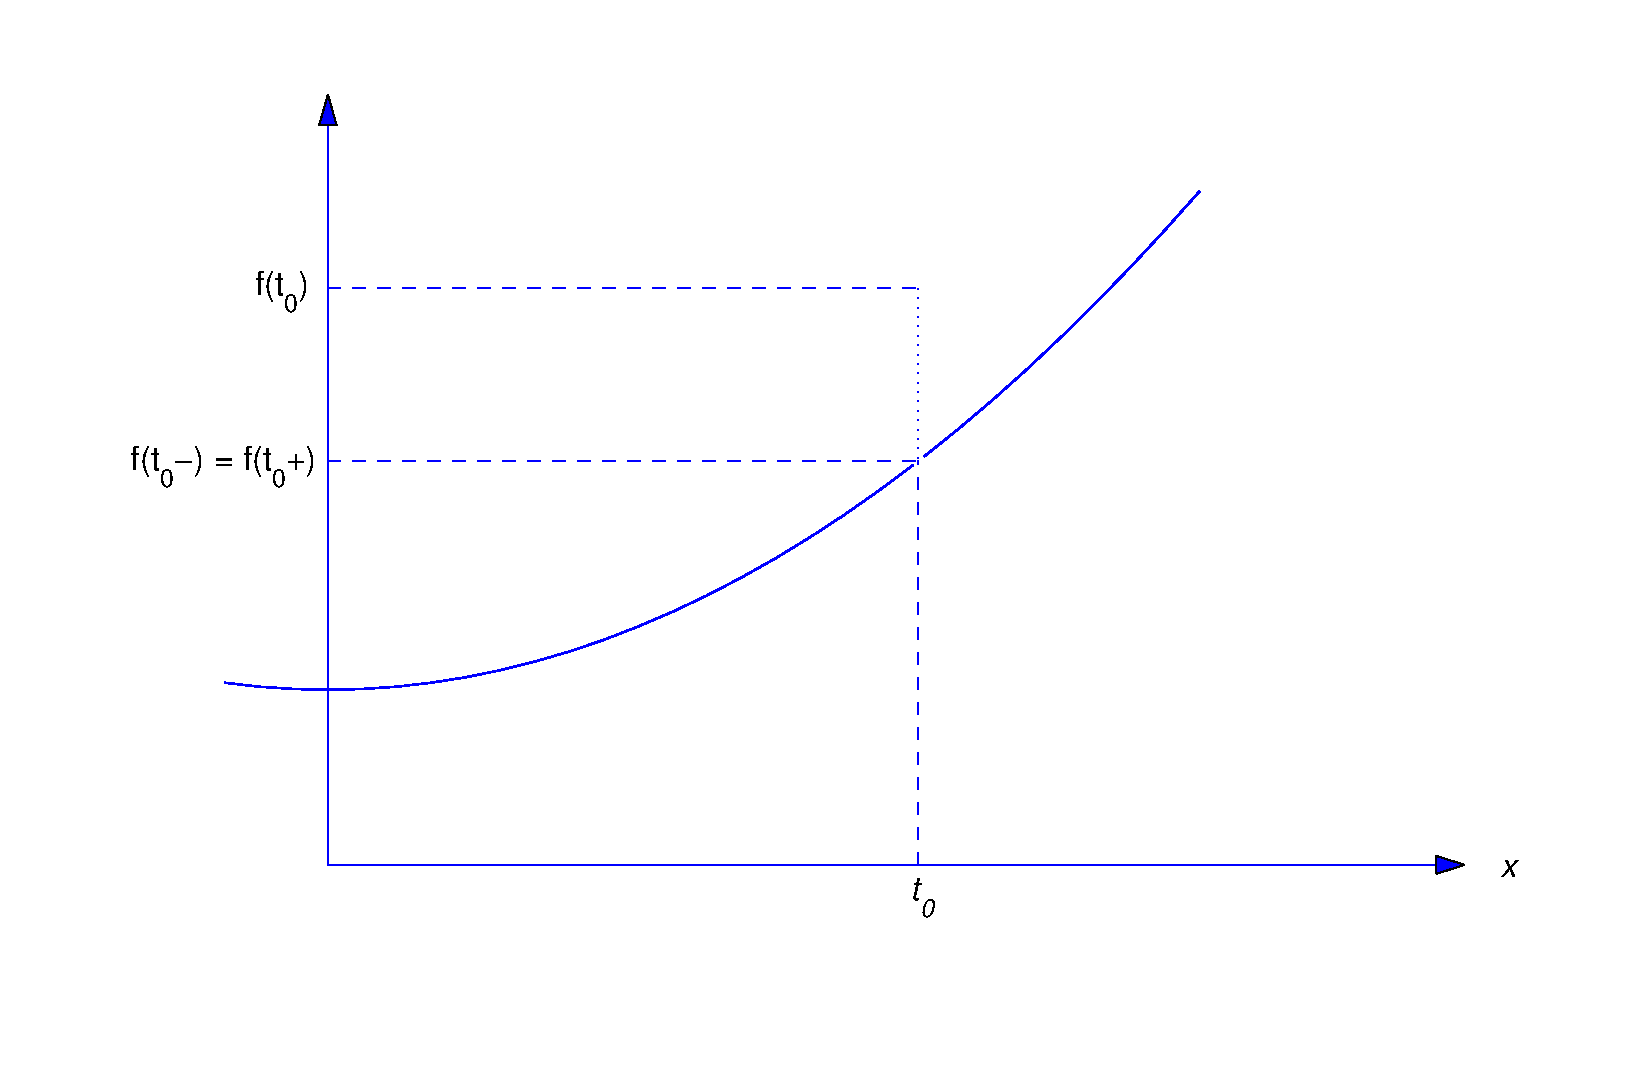
\includegraphics[bb=-78 148 689 643,width=5.67in,height=3.66in,keepaspectratio]{fig080102}}
  \caption{}
  \label{figure:8.1.2}
\end{minipage}
  \begin{minipage}[b]{0.5\linewidth}
    \centering
   \scalebox{.65}{
  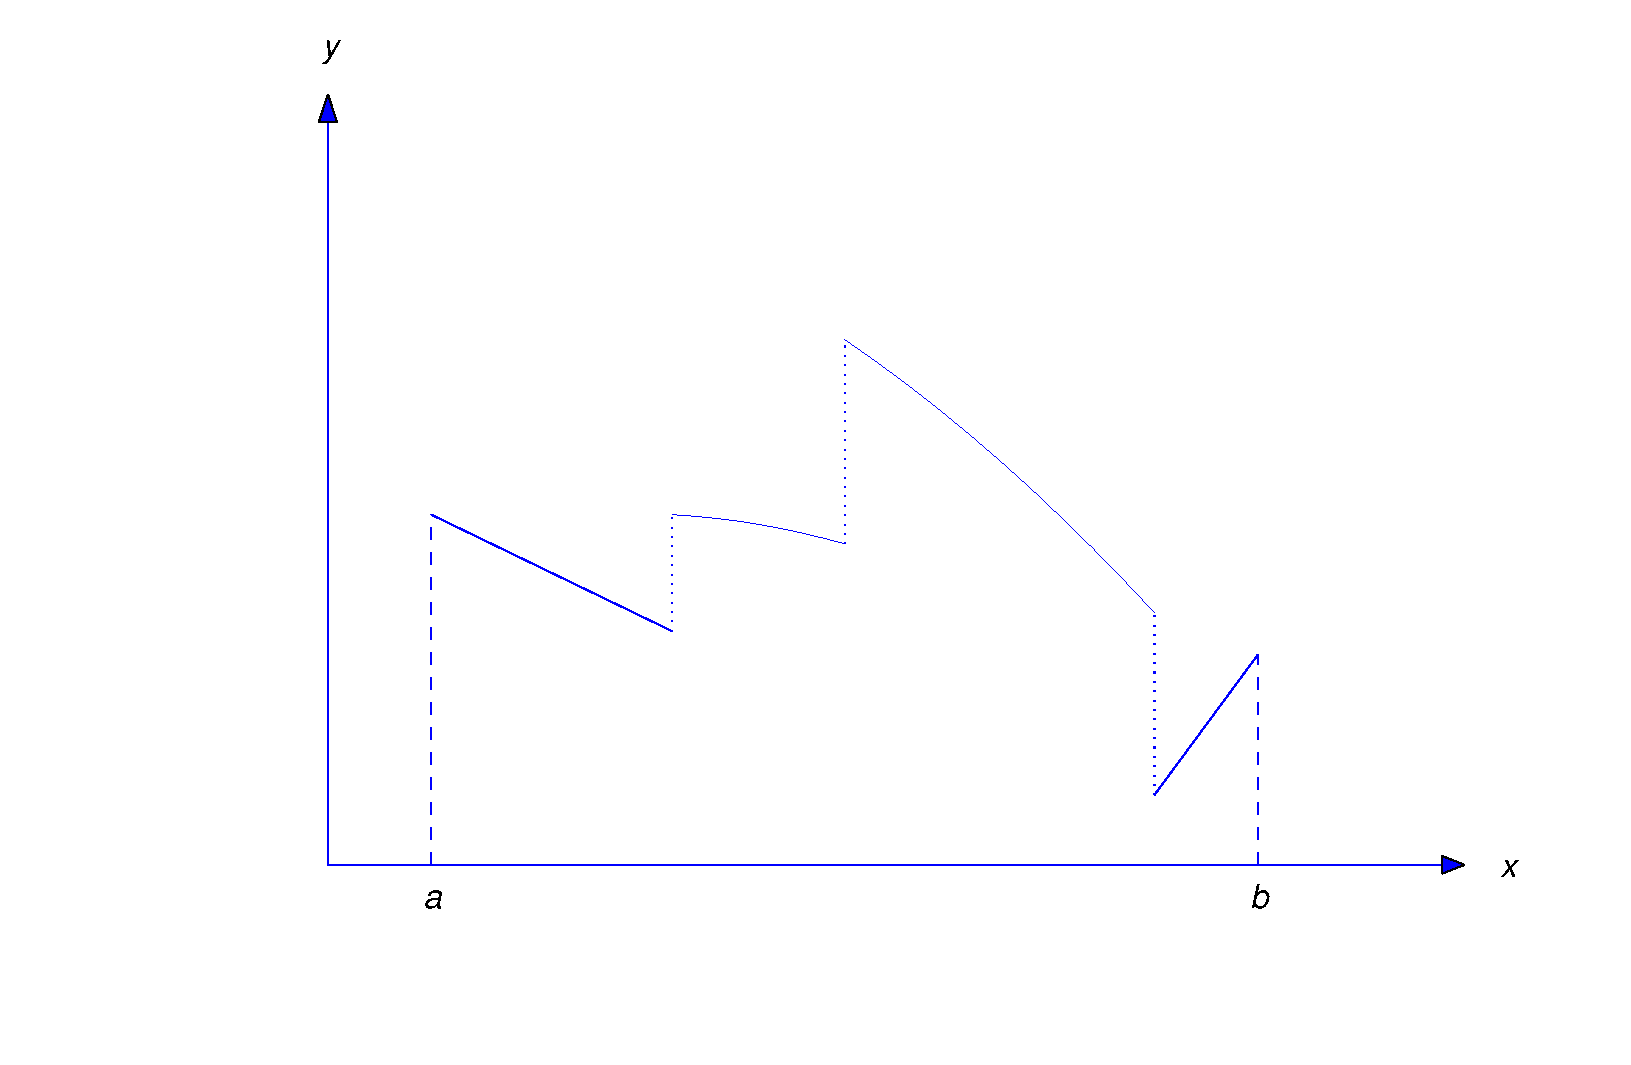
\includegraphics[bb=-78 148 689 643,width=5.67in,height=3.66in,keepaspectratio]{fig080103}}
\caption{A piecewise continuous function on $[a,b]$}
  \label{figure:8.1.3}
\end{minipage}
\end{figure}

\color{blue}
\remark{We know from calculus that a definite integral isn't
affected by changing the values of its integrand at isolated points.
Therefore, redefining a function $f$ to make it continuous at
removable discontinuities does not change ${\cal L}(f)$.}
\color{black}

\begin{definition}\color{blue}\label{thmtype:8.1.4}\rm
\mbox{}
\begin{rmlist}
\item % (i)
A function $f$ is said to be {\color{blue}\it piecewise continuous} on a finite
closed interval $[0,T]$ if $f(0+)$ and $f(T-)$ are finite and $f$ is
continuous on the open interval $(0,T)$ except possibly at finitely
many points, where $f$ may have jump discontinuities or removable
discontinuities.
\item % (ii)
A function $f$ is said to be {\color{blue}\it piecewise continuous} on the
infinite interval $[0,\infty)$ if it's piecewise continuous on
$[0,T]$ for every $T>0$.
\end{rmlist}
\end{definition}

Figure~\ref{figure:8.1.3} shows the graph of a typical piecewise
continuous function.

It is shown in calculus that if a function is piecewise continuous on
a finite closed interval then it's integrable on that interval. But
if $f$ is piecewise continuous on $[0,\infty)$, then so is $e^{-st}f
(t)$, and therefore
$$
\int_0^T e^{-st}f(t)\,dt
$$
exists for every $T>0$. However, piecewise continuity alone does not
guarantee that the improper integral
\begin{equation}\label{eq:8.1.13}
\int_0^\infty e^{-st}f(t)\,dt=\lim_{T\to\infty}\int_0^T e^{-st}f(t)\,
dt
\end{equation}
converges for $s$ in some interval $(s_0,\infty)$. For example, we
noted earlier that \eqref{eq:8.1.13} diverges for all $s$ if
$f(t)=e^{t^2}$. Stated informally, this occurs because $e^{t^2}$
increases too rapidly as $t\to\infty$. The next definition
provides a constraint on the growth of a function that guarantees
convergence of its Laplace transform for $s$ in some interval
$(s_0,\infty)$ .

\begin{definition}\color{blue}\label{thmtype:8.1.5}\rm A
function $f$ is said to be
{\color{blue}\it of exponential order\/} $s_0$ if there are constants $M$ and $t_0$
such that
\begin{equation}\label{eq:8.1.14}
|f(t)|\le Me^{s_0t},\quad t\ge t_0.
\end{equation}
In situations where the specific value of $s_0$
is irrelevant we say simply that $f$ is {\color{blue}\it of exponential order\/}.
\end{definition}

The next theorem gives useful sufficient conditions for a function $f$
to have a Laplace transform.  The proof is sketched in
Exercise~\ref{exer:8.1.10}.

\begin{theorem}\color{blue}\label{thmtype:8.1.6} If $f$
is piecewise continuous on $[0,\infty)$ and of exponential order $s_0$,
 then ${\cal L}(f)$ is defined for $s>s_0$.
\end{theorem}

\color{blue}
\remark{
We emphasize that the conditions of Theorem~\ref{thmtype:8.1.6}
 are sufficient, but {\color{blue}\it not necessary\/}, for $f$ to have a Laplace
transform. For example, Exercise~\ref{exer:8.1.14}\part{c} shows that  $f$
may have a Laplace transform even though $f$ isn't  of exponential
order.}
\color{black}

\begin{example}\label{example:8.1.8}\rm
If $f$ is bounded on some interval $[t_0,\infty)$, say
$$
|f(t)|\le M,\quad t\ge t_0,
$$
then \eqref{eq:8.1.14} holds with $s_0=0$, so $f$ is of exponential order
zero. Thus, for example, $\sin\omega t$ and $\cos \omega t$ are of
exponential order zero, and Theorem~\ref{thmtype:8.1.6} implies that
${\cal L}(\sin\omega t)$ and ${\cal L}(\cos \omega t)$ exist for
$s>0$. This is consistent with the conclusion of
Example~\ref{example:8.1.4}.
\end{example}

\begin{example}\label{example:8.1.9}\rm
It can be shown that if $\lim_{t\to\infty}e^{-s_0t}f(t)$ exists and is
finite then $f$ is of exponential order $s_0$
(Exercise~\ref{exer:8.1.9}). If $\alpha$ is any real number and $s_0>0$
then $f(t)=t^\alpha$ is of exponential order $s_0$, since
$$
\lim_{t\to\infty}e^{-s_0t}t^\alpha=0,
$$
by L'H\^opital's rule. If $\alpha\ge 0$, $f$ is also
continuous on $[0,\infty)$. Therefore Exercise~\ref{exer:8.1.9} and
Theorem~\ref{thmtype:8.1.6} imply that ${\cal L}(t^\alpha)$ exists for
$s\ge s_0$. However, since $s_0$ is an arbitrary positive number, this
really implies that ${\cal L}(t^\alpha)$ exists for all $s>0$. This is
consistent with the results of Example~\ref{example:8.1.2} and
Exercises~\ref{exer:8.1.6} and \ref{exer:8.1.8}.
\end{example}

\begin{example}\label{example:8.1.10}\rm
Find the Laplace transform of the piecewise continuous function
$$
f(t)=\left\{\begin{array}{cl} 1,&0\le t<1,\\  -3e^{-t},&t\ge
1.\end{array}\right.
$$
\end{example}

\solution    Since $f$ is defined by different formulas
on $[0,1)$ and $[1,\infty)$, we write
$$
 F(s)=\int_0^\infty e^{-st} f(t)\,dt
=\int_0^1e^{-st}(1)\,dt+\int_1^\infty
e^{-st}(-3e^{-t})\,dt.
$$
Since
$$
\int_0^1e^{-st}\,dt=\left\{\begin{array}{cl}\dst{{1-e^{-s}\over
s}},&\quad s\ne0,\\[2\jot] 1,&\quad s=0,\end{array}\right.
$$
 and
$$
\int_1^\infty e^{-st}(-3e^{-t})\,dt=-3\int_1^\infty
e^{-(s+1)t}\,dt=-{3e^{-(s+1)}\over s+1},\quad s>-1,
$$
it follows that
$$
F(s)=\left\{\begin{array}{rl}\dst{{1-e^{-s}\over
s}-3{e^{-(s+1)}\over
s+1}},&s>-1,\,s\ne0,\\\hfill\dst{1-{3\over e}}\hfill,&
s=0.\end{array}\right.
$$
This is consistent with Theorem~\ref{thmtype:8.1.6}, since
$$
|f(t)|\le 3e^{-t},\quad  t\ge 1,
$$
and therefore $f$ is of exponential order $s_0=-1$.

\color{blue}
\remark{In Section~8.4 we'll develop a more efficient
method for finding Laplace transforms of piecewise continuous
functions.}
\color{black}

\begin{example}\label{example:8.1.11}\rm
We stated  earlier that
$$
\int_0^\infty e^{-st} e^{t^2} dt=\infty
$$
for all $s$, so Theorem~\ref{thmtype:8.1.6} implies that $f(t)=e^{t^2}$
is not  of exponential order, since
$$
\lim_{t\to\infty} {e^{t^2}\over Me^{s_0t}}=\lim_{t\to\infty} {1\over
M} e^{t^2-s_0t}=\infty,
$$
so
$$
e^{t^2}>Me^{s_0t}
$$
for sufficiently large values of $t$, for any choice of $M$ and $s_{0}$
(Exercise~\ref{exer:8.1.3}).
\end{example}

\exercises

\begin{exerciselist}
\item\label{exer:8.1.1}
Find the Laplace transforms of the following functions by evaluating
the integral $F(s)=\int_0^\infty e^{-st} f(t)\,dt$.

\begin{tabular}[t]{@{}p{112pt}@{}p{112pt}@{}p{112pt}}
\part{a} $t$  & \part{b} $te^{-t}$ & \part{c} $\sinh bt$\\
 \part{d} $e^{2t}-3e^t$  & \part{e} $t^2$
\end{tabular}

\item\label{exer:8.1.2}
Use  the table of Laplace transforms to
find the Laplace transforms of the following functions.

\begin{tabular}[t]{@{}p{112pt}@{}p{112pt}@{}p{112pt}}
\part{a}  $\cosh t\sin t$ & \part{b}  $\sin^2t$ & \part{c}  $\cos^2
2t$\\ \part{d}  $\cosh^2 t$ & \part{e}  $t\sinh 2t$ & \part{f}
$\sin
t\cos t$\\ \part{g}  $\dst{\sin\left(t+{\pi\over
4}\right)}$ & \part{h}  $\cos 2t -\cos 3t$ & \part{i}  $\sin 2t +\cos
4t$
\end{tabular}

\item\label{exer:8.1.3}
 Show that
$$
\int_0^\infty e^{-st}e^{t^2} dt=\infty
$$
for every real number $s$.

\item\label{exer:8.1.4}
 Graph the following piecewise continuous functions and evaluate
$f(t+)$, $f(t-)$, and $f(t)$ at each point of discontinuity.

\begin{tabular}[t]{@{}p{168pt}@{}p{168pt}}
\part{a} $f(t)=\left\{\begin{array}{cl} -t,
& 0\le t<2,\\ t-4, & 2\le t<3,\\ 1, & t\ge
3.\end{array}\right.$ &
\part{b} $f(t)=\left\{\begin{array}{cl} t^2+2, & 0
\le t<1,\\4, & t=1,\\ t, & t>
1.\end{array}\right.$\\[15pt]
\part{c} $f(t)=\left\{\begin{array}{rl}
\sin t, & 0\le t<\pi/ 2,\\ 2\sin t, &\pi/ 2
\le t<\pi,\\ \cos t, & t\ge\pi.\end{array}\right.$ &
\part{d} $f(t)=\left\{\begin{array}{cl}t,
 & 0\le t<1,\\ 2, & t=1,\\ 2-t, & 1
\le t<2,\\ 3, & t=2,\\ 6, & t>
2.\end{array}\right.$
\end{tabular}

\item\label{exer:8.1.5}
 Find the Laplace transform:

\begin{tabular}[t]{@{}p{168pt}@{}p{168pt}}
\part{a} $f(t)=\left\{\begin{array}{rl} e^{-t}, &
0\le t<1,\\ e^{-2t}, & t\ge 1.\end{array}\right.$ &
\part{b} $f(t)=\left\{\begin{array}{rl} 1, & 0\le t<
4,\\ t, & t\ge 4.\end{array}\right.$\\[2\jot]
\part{c} $f(t)=\left\{\begin{array}{rl} t, & 0\le
t<1,\\ 1, & t\ge 1.\end{array}\right.$&
\part{d}  $f(t)=\left\{\begin{array}{rl} te^t, & 0\le
t<1,\\\phantom{t} e^t, & t\ge 1.\end{array}\right.$
\end{tabular}

\item\label{exer:8.1.6}
Prove that if $f(t)\leftrightarrow F(s)$ then $t^kf(t)\leftrightarrow
(-1)^kF^{(k)}(s)$. \hint{Assume that it's permissible to differentiate
the integral $\int_0^\infty e^{-st}f(t)\,dt$ with respect to $s$ under
the integral sign.}

\item\label{exer:8.1.7}
Use the known Laplace transforms
$$
{\cal L}(e^{\lambda t}\sin\omega t)={\omega\over(s-\lambda)^2+\omega^2}
\quad\mbox{and }\quad
{\cal L}(e^{\lambda t}\cos\omega t)={s-\lambda\over(s-\lambda)^2+\omega^2}
$$
  and the result of Exercise~\ref{exer:8.1.6} to find
${\cal L}(te^{\lambda t}\cos\omega t)$ and
${\cal L}(te^{\lambda t}\sin\omega t)$.

\item\label{exer:8.1.8}
 Use the known Laplace transform ${\cal L}(1)=1/s$ and the result of
Exercise~\ref{exer:8.1.6} to show that
$$
{\cal L}(t^n)={n!\over s^{n+1}},\quad n=\mbox{ integer}.
$$

\item\label{exer:8.1.9}
\begin{alist}
\item % (a)
 Show that if $\lim_{t\to\infty} e^{-s_0t} f(t)$ exists and
is finite then  $f$ is of exponential order $s_0$.
\item % (b)
 Show that if $f$ is of exponential order $s_0$ then $\lim_{t
\to\infty} e^{-st} f(t)=0$ for all $s>s_0$.
\item % (c)
Show that if $f$ is of exponential order $s_0$  and $g(t)=f(t+\tau)$
where $\tau>0$, then $g$ is also of exponential order $s_0$.
\end{alist}

\item\label{exer:8.1.10}
Recall the next  theorem from calculus.

\color{blue}
{\sc Theorem A.} \it Let $g$ be integrable on $[0,T]$ for
every $T>0$.  Suppose there's a function $w$ defined on some
interval $[\tau,\infty)$ (with $\tau\ge 0$) such that $|g(t)|\le
w(t)$ for $t\ge\tau$ and $\int^\infty_\tau w(t)\,dt$
converges.  Then $\int_0^\infty g(t)\,dt$ converges.\rm
\color{black}

Use Theorem A to show that if $f$ is piecewise continuous on
$[0,\infty)$ and of exponential order $s_0$, then $f$ has a Laplace
transform $F(s)$ defined for $s>s_0$.

\item\label{exer:8.1.11}
 Prove: If $f$ is piecewise continuous and of exponential order
then $\lim_{s\to\infty}F(s)~=~0$.

\item\label{exer:8.1.12}
Prove: If $f$ is continuous on $[0,\infty)$ and of exponential order
$s_0>0$, then
$$
{\cal L}\left(\int^t_0 f(\tau)\,d\tau\right)={1\over s} {\cal L} (f),
\quad s>s_0.
$$
\hint{Use integration by parts to evaluate the transform on
the left.}

\item\label{exer:8.1.13}
Suppose $f$ is piecewise continuous and of exponential
order, and that $\lim_{t\to 0+} f(t)/t$ exists.  Show that
$$
{\cal L}\left({f(t)\over t}\right)=\int^\infty_s F(r)\,dr.
$$
\hint{Use  the results of Exercises~$6$ and $11$.}

\item\label{exer:8.1.14}
Suppose $f$ is piecewise continuous on $[0,\infty)$.
\begin{alist}
\item % (a)
Prove: If the integral $g(t)=\int^t_0 e^{-s_0\tau} f(\tau)\,d\tau$
satisfies the inequality $|g(t)|\le M\; (t\ge 0)$, then $f$ has a
Laplace transform $F(s)$ defined for $s>s_0$. \hint{Use integration by
parts to show that
$$
\int_0^T e^{-st}f(t)\,dt = e^{-(s-s_0)T}g(T)
+(s-s_0)\int_0^Te^{-(s-s_0)t}g(t)\,dt.
$$}
\item % (b)
 Show that if ${\cal L}(f)$ exists for
$s=s_0$ then it exists for $s>s_0$.
Show that the function
$$
f(t)=te^{t^2}\cos(e^{t^2})
$$
has a Laplace transform defined for $s>0$, even though $f$ isn't  of
exponential order.
\item % (c)
Show that the function
$$
f(t)=te^{t^2}\cos(e^{t^2})
$$
has a Laplace transform defined for $s>0$, even though $f$ isn't  of
exponential order.
\end{alist}

\item\label{exer:8.1.15}
Use the table of Laplace transforms and the result of
Exercise~\ref{exer:8.1.13} to find the Laplace transforms of the following
functions.

\begin{tabular}[t]{@{}p{112pt}@{}p{112pt}@{}p{112pt}}
\part{a} $\dst{{\sin\omega t\over t}\quad(\omega>0)}$ &
\part{b} $\dst{{\cos\omega t-1\over t}}\quad (\omega>0)$ &
\part{c} $\dst{{e^{at}-e^{bt}\over t}}$\\[2\jot]
\part{d} $\dst{{\cosh t-1\over t}}$ &
\part{e} $\dst{{\sinh^2 t\over t}}$
\end{tabular}

\item\label{exer:8.1.16}
  The {\color{blue}\it gamma function} is defined by
$$
\Gamma (\alpha)=\int_0^\infty x^{\alpha-1}e^{-x}\,dx,
$$
which can be shown to converge if $\alpha>0$.
\begin{alist}
\item % (a)
 Use integration by parts to show that
$$
\Gamma (\alpha+1)=\alpha\Gamma (\alpha),\quad\alpha>0.
$$
\item % (b)
 Show that $\Gamma(n+1)=n!$ if $n=1$, $2$, $3$,\dots.
\item % (c)
 From  \part{b} and the table of Laplace transforms,
$$
{\cal L}(t^\alpha)={\Gamma (\alpha+1)\over s^{\alpha+1}},\quad s>0,
$$
if $\alpha$ is a nonnegative integer.  Show that this formula is valid for
any $\alpha>-1$. \hint{Change the variable of integration in the
integral for $\Gamma (\alpha+1)$.}
\end{alist}

\item\label{exer:8.1.17}
  Suppose $f$ is continuous on $[0, T]$ and $f(t+T)=f(t)$
for all $t\ge 0$.  (We say in this case that $f$ is {\color{blue}\it periodic with
period\/} $T$.)
\begin{alist}
\item % (a)
 Conclude from Theorem~\ref{thmtype:8.1.6} that the Laplace transform of
$f$ is defined for $s>0$. \hint{Since $f$ is
continuous on $[0,T]$ and periodic with period $T$, it's bounded
on $[0,\infty)$.}
\item % (b)
 \part{b} Show that
$$
F(s)={1\over 1-e^{-sT}}\int_0^T e^{-st}f(t)\,dt,\quad s>0.
$$
\hint{Write
$$
F(s)=\sum^\infty_{n=0}\int^{(n+1)T}_{nT}e^{-st} f(t)\,dt.
$$
Then show that
$$
\int^{(n+1)T}_{nT} e^{-st}f(t)\,dt=e^{-nsT}\int_0^T e^{-st}f(t)\,dt,
$$
and recall the formula for the sum of a geometric series.}
\end{alist}

\item\label{exer:8.1.18}
  Use the formula given in Exercise~\ref{exer:8.1.17}\part{b} to find
the
Laplace transforms of the given periodic functions:
\begin{alist}
\item % (a)
 $\dst{f(t)=\left\{\begin{array}{cl} t, & 0\le
t<1,\\ 2-t, & 1\le t<2,\end{array}\right.\hskip30pt f(t+2)=f(t),
\quad t\ge 0}$
\item % (b)
 $\dst{f(t)=\left\{\begin{array}{rl}1, & 0\le
t<{1\over 2},\\ -1, & {1\over 2}\le t<1,\end{array}\right.
\hskip30pt f(t+1)=f(t),\quad t\ge 0}$
\item % (c)
 $f(t)=|\sin t|$
\item % (d)
 $\dst{f(t)=\left\{\begin{array}{cl}\sin t, & 0\le t<
\pi,
\\ 0, &\pi\le t<2\pi,\end{array}\right.\hskip30pt
f(t+2\pi)=f(t)}$
\end{alist}

\end{exerciselist}
